%%=============================================================================
%% Proof of concept
%%=============================================================================
\chapter{Proof of concept}
\label{ch:proof-of-concept}

\section{Doelstelling van de PoC}

%Wat wil je bewijzen of aantonen met deze PoC?
De hoofddoelstelling van deze PoC is om na te gaan op welke manier een LLM ondersteuning kan bieden binnen een IT-supportsysteem. Er werden verschillende benaderingen onderzocht, maar uit de analyse bleek dat RAG de meest geschikte aanpak is. 
\\[1em]
%Welke hypothese test je eigenlijk?
De hypothese die binnen deze PoC getest wordt, kan als volgt worden samengevat:
\textit{“Een LLM, gecombineerd met Retrieval-Augmented Generation (RAG), kan effectief en efficiënt ondersteuning bieden binnen een IT-supportsysteem door relevante informatie uit documentatie te halen en daarmee het supportproces te optimaliseren en te vereenvoudigen.”}

\section{Behoeften analyse}
Voor de PoC werd een MoSCoW-analyse uitgevoerd om de functionele vereisten te prioritiseren.
De analyse werd onderverdeeld in \textit{Must haves}, \textit{Should haves} en \textit{Could haves}

\subsection{Must haves}
\begin{itemize}
    \item \textbf{Vragen kunnen stellen in de eigen taal (bijvoorbeeld Nederlands, Frans en Engels)}:\\ 
    Het systeem moet correct functioneren ongeacht of de gebruiker vragen stelt in het Nederlands, Frans of Engels.
    \item \textbf{Een duidelijk en bruikbaar antwoord ontvangen op basis van betrouwbare bronnen}:\\ 
    De gegenereerde antwoorden moeten informatief, relevant en praktisch toepasbaar zijn.
    \item \textbf{Eenvoudige en intuïtieve interface}:\\  
    De gebruiker mag geen technische kennis nodig hebben; de interactie moet vanzelfsprekend en gebruiksvriendelijk aanvoelen.
    \item \textbf{Consistente ervaring (snel, zonder fouten of willekeurige antwoorden)}:\\  
    De gebruiker verwacht dat de applicatie betrouwbaar functioneert en consistente resultaten levert.
\end{itemize}

\subsection{Should haves}
\begin{itemize}
    \item \textbf{Het systeem begrijpt vervolgvragen binnen een sessie}:\\  
    De gebruiker moet een gesprek kunnen voeren waarbij eerdere vragen worden meegenomen in de context, zodat interacties natuurlijker verlopen.
    \item \textbf{Mogelijkheid om feedback te geven op het antwoord}:\\  
    De gebruiker kan aangeven of een antwoord onjuist is of dat er meer detail gewenst is, bijvoorbeeld met opties zoals “Dit antwoord klopt niet” of “Ik wil meer detail”.
    \item \textbf{Transparantie over de gebruikte bronnen van het antwoord}:\\  
    De gebruiker moet kunnen zien uit welk document of welke bron het antwoord afkomstig is, zodat de informatie steeds gecontroleerd en gevalideerd kan worden.
\end{itemize}

\subsection{Could haves}
\begin{itemize}
    \item \textbf{Langetermijngeheugen over meerdere sessies heen}:\\  
    Het opzetten van een geheugen dat sessie-overstijgend werkt, brengt extra complexiteit met zich mee en is daarom minder geschikt voor een eerste versie.
    \item \textbf{Zelf documenten kunnen uploaden of bewerken}:\\  
    In deze PoC ligt de focus op het zoeken en beantwoorden van vragen, niet op het beheren van documenten.
    \item \textbf{Automatisch mails behandelen}:\\  
    Het automatisch verwerken en beantwoorden van e-mails valt qua complexiteit buiten de scope van een eerste versie.
\end{itemize}

\section{Architectuur en Ontwerp}

\subsection{Algemene structuur}

Deze structuur bestaat uit een graaf die is opgebouwd uit verschillende knooppunten (nodes). De graaf stelt het LLM bovendien in staat om zelfstandig te bepalen welke keuzes gemaakt moeten worden tijdens het verwerken van een vraag.
\\[1em]
De standaard RAG-architectuur gaat een query gaan embedden en haalt vervolgens de meest relevante documenten op uit de vectordatabase, zonder verdere reflectie over de nood van het ophalen van de documenten en de werkelijke relevantie van deze documenten. Hoewel dit op het eerste gezicht een efficiënte aanpak lijkt, betekent het ook dat het systeem bij elke willekeurige gebruikersvraag opnieuw de vectordatabase bevraagt, zelfs wanneer dat niet noodzakelijk is.
\\[1em]
Om dit te vermijden, werd gebruikgemaakt van een graafstructuur die de LLM de mogelijkheid geeft om zelf te beoordelen wanneer het relevant is om documenten op te halen. Daarnaast wordt de LLM ook verantwoordelijk geacht om te oordelen over de opgehaalde documenten. De volledige flow van het proces kan worden bekeken in figuur~\ref{fig:Architectuur}
\\[1em]
De PoC werd uitgewerkt met behulp van Ollama, een tool waarmee open modellen lokaal kunnen worden gedraaid. Tijdens overleg met de betrokken partijen werd geen voorkeur uitgesproken voor specifieke LLM-modellen, enkel het gebruik van DeepSeek werd afgeraden.

\begin{figure}[H]
    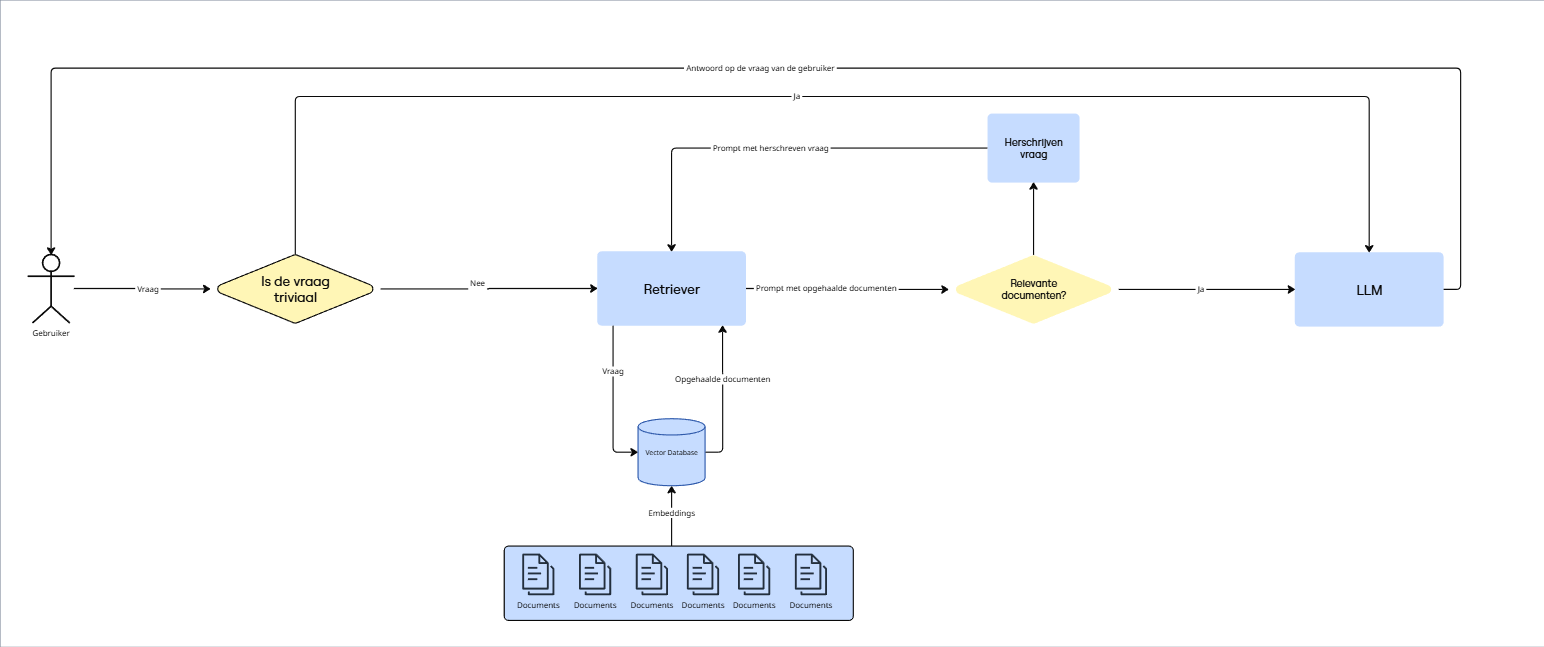
\includegraphics[width=1\textwidth]{flowchart.png}
    \caption{Architectuur van de PoC op basis van een graafgebaseerde workflow}
    \label{fig:Architectuur}
\end{figure}

%Belangrijke keuzes tijdens het bouwen (waarom bv. technologie X en niet Y?).

Een van de belangrijkste beslissingen in deze PoC was de initiële keuze voor RAG ten opzichte van andere mogelijke benaderingen. Eens deze keuze gemaakt was, volgde de selectie van een geschikt framework om RAG te implementeren.
\\[1em]
Voor deze PoC werd gekozen voor LangGraph, een framework waarmee zogenaamde agents kunnen worden opgebouwd aan de hand van grafen. Dit verschilt van bijvoorbeeld LangChain, waar gewerkt wordt met ketens van opeenvolgende stappen.
\\[1em]
LangGraph biedt meer flexibiliteit in het aansturen van de flow en logica binnen het systeem. Zo kan een LLM bijvoorbeeld zelf kiezen welke paden in de graaf doorlopen worden, of kan er een lus geïntroduceerd worden binnen de graafstructuur. Beide mechanismen werden effectief toegepast in deze PoC.
\\[1em]
%Welke tools, frameworks, programmeertalen gebruik je?
Hieronder een overzicht van de verschillende frameworks, tools en programmeertalen die werden gebruikt om deze PoC op te stellen.
\\[1em]
\textbf{Frameworks/libraries:}
\begin{itemize}
    \item Langchain
    \item LangGraph
    \item Streamlit
    \item Ragas
\end{itemize}

\textbf{Tools:}
\begin{itemize}
    \item ChromaDB
    \item Ollama
\end{itemize}

\textbf{Programmeertalen:}
\begin{itemize}
    \item Python
\end{itemize}

%Schema’s (bv. systeemdiagram, flowchart) zijn hier heel sterk.

\subsection{Implementatie}

%Hoe heb je de POC concreet opgebouwd?
\subsubsection{vectorstore}
De PoC werd opgebouwd volgens de klassieke RAG-implementatie. In de eerste fase werden de originele documenten opgesplitst in kleinere tekstsegmenten en vervolgens omgezet naar embeddings via een vooraf getraind embedding model. Voor deze PoC werd hiervoor gebruikgemaakt van het \verb|mxbai-embed-large model|. Van de beschikbare embedding modellen binnen Ollama biedt dit model de hoogste semantische nauwkeurigheid.

\begin{lstlisting}[basicstyle=\small, frame=single, breaklines=true, postbreak=\mbox{\textcolor{red}{$\hookrightarrow$}\space}, escapeinside ={\%,}, escapechar={!}, numbers=left, language=Python, caption=Embedding model]
def get_embedding():
    return OllamaEmbeddings(model='mxbai-embed-large')
\end{lstlisting}

Gekoppeld aan het embedding model is er ook een chatmodel dat doorheen het proces wordt gebruikt. De variabele \verb|response_model_name| bepaalt welk model wordt gebruikt tijdens de flow. De enige configuratie die werd aangepast, is het instellen van de temperatuur op nul. De temperatuur bepaalt hoe creatief het model zal zijn in zijn antwoorden. Aangezien het de bedoeling is om zo weinig mogelijk hallucinaties te veroorzaken, werd ervoor gekozen om deze waarde op nul te zetten.

\begin{lstlisting}[basicstyle=\small, frame=single, breaklines=true, postbreak=\mbox{\textcolor{red}{$\hookrightarrow$}\space}, escapeinside ={\%,}, escapechar={!},
numbers=left, language=Python, caption=Chat model]
def get_response_model():
    return ChatOllama(model=response_model_name, temperature=0)
\end{lstlisting}



Elke chunk heeft een grootte van 1250 karakters, met een overlap van 250 karakters tussen opeenvolgende chunks. Na het testen van verschillende chunk groottes bleek dit de kleinst mogelijke waarde te zijn waarbij nog voldoende relevante informatie kon worden opgehaald.

\begin{lstlisting}[basicstyle=\small, frame=single, breaklines=true, postbreak=\mbox{\textcolor{red}{$\hookrightarrow$}\space}, escapeinside ={\%,}, escapechar={!}, numbers=left, language=Python, caption=Vector store build] 
# Split the document into chunks
text_splitter = RecursiveCharacterTextSplitter(chunk_size=1250, chunk_overlap=250)
docs = text_splitter.split_documents(documents)
\end{lstlisting}

De gegenereerde embeddings worden vervolgens opgeslagen in een vectorstore. Hiervoor werd gekozen voor ChromaDB, een performante oplossing. Alternatieven zoals Faiss zijn zeker ook mogelijk.

\begin{lstlisting}[basicstyle=\small, frame=single, breaklines=true, postbreak=\mbox{\textcolor{red}{$\hookrightarrow$}\space}, escapeinside ={\%,}, escapechar={!}, numbers=left, language=Python, caption=Vector store build]
# Return a ChromaDB instance
return (Chroma.from_documents(
        docs, embeddings_function, persist_directory=persistent_directory)
        .as_retriever(search_type=search_type, search_kwargs=search_kwargs))
\end{lstlisting}

Deze initiële set-up maakt het mogelijk om relevante documenten snel op te halen op basis van semantische gelijkenis met de vraag van de gebruiker. Met andere woorden: dit vormt een kerncomponent van de RAG-oplossing.

\subsubsection{Graaf structuur en nodes}

Eens de vector met de nodige documenten beschikbaar is kunnen er vragen gesteld worden aan de LLM die aan de hand van een graaf keuzes zal maken naargelang de vraag van de gestelde gebruiker. De volledige workflow werd gemodelleerd als een LangGraph-graaf. Deze structuur is weergegeven in figuur~\ref{fig:langgraph}.

\begin{figure}[H]
    \centering
    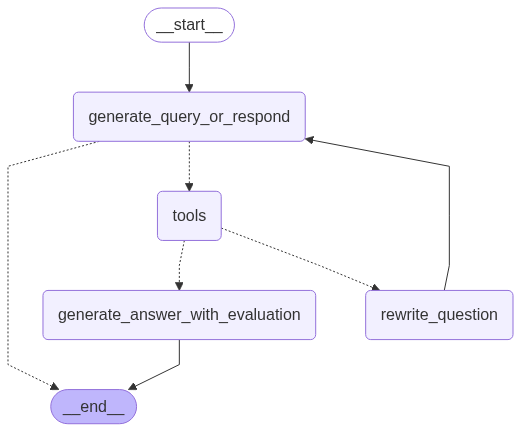
\includegraphics[width=0.8\textwidth]{langgraph_workflow.png}
    \caption{Technische uitwerking van de workflow als LangGraph-graaf}
    \label{fig:langgraph}
\end{figure}

\paragraph{Antwoorden of documenten ophalen}

Vooraleer het RAG-proces op gang wordt gebracht, moet de LLM eerst een inschatting maken van de vraag die de gebruiker heeft gesteld. Wanneer het gaat om een triviale vraag of een eenvoudig bericht, dient de LLM onmiddellijk een antwoord te geven, zonder het volledige RAG-proces te doorlopen.
\\[1em]
Om dit te realiseren, wordt gebruikgemaakt van de volgende prompt, waarin de input van de gebruiker wordt ingevuld: 

\begin{lstlisting}[basicstyle=\small, frame=single, breaklines=true, postbreak=\mbox{\textcolor{red}{$\hookrightarrow$}\space}, escapeinside ={\%,}, escapechar={!}, numbers=left, language=Python, caption=Prompt retrieve or respond]
RETRIEVE_DOCUMENTS_OR_RESPOND_PROMPT = """
    This method decides whether to call the retriever tool or respond directly.
    
    If the user's question is trivial, respond directly. Just respond directly. Do not show your reasoning or thinking process.
    If the question is non-trivial, use the retriever tool to generate a response.
    If in doubt, use the retriever tool to make sure.
    
    Given the user's question:  
    "{message}"
    
    Determine whether the question is trivial. 
"""
\end{lstlisting}

Het voordeel van deze aanpak is dat er geen onnodige resources worden verbruikt bij het uitvoeren van het RAG-proces. Enkel wanneer de vraag van de gebruiker effectief nood heeft aan specifieke contextuele informatie, wordt de retriever geactiveerd.
\\[1em]
De LLM krijgt een retriever tool ter beschikking en kan vervolgens autonoom beslissen of deze tool wordt gebruikt of dat er meteen een antwoord gegenereerd wordt. Dit gedrag wordt geïmplementeerd in de volgende node:

\begin{lstlisting}[basicstyle=\small, frame=single, breaklines=true, postbreak=\mbox{\textcolor{red}{$\hookrightarrow$}\space}, escapeinside ={\%,}, escapechar={!}, numbers=left, language=Python, caption=Node die keuze maakt tussen om al dan niet te retrieven]
def retrieve_documents_or_respond(state: MessagesState) -> MessagesState:
    """
    This methods will call the retriever tool when given a non trivial question is asked.
    In the case of a trivial question it will simply provide a response
    Call the model to generate a response based on the current state. Given
    the question, it will decide to retrieve using the retriever tool, or simply respond to the user.
    """
    message = state["messages"][-1].content
    
    prompt = RETRIEVE_DOCUMENTS_OR_RESPOND_PROMPT.format(message=message)
    
    response_model_with_tools = response_model.bind_tools([myminfin_retriever_tool])
    response = response_model_with_tools.invoke([SystemMessage(content=prompt),
    HumanMessage(content=message)])
    return MessagesState(messages=[response])
\end{lstlisting}

\paragraph{Retriever}

Zodra de keuze wordt gemaakt om documenten op te halen, roept het LLM-model de retriever-tool aan. Deze tool raadpleegt ChromaDB om, op basis van een vooraf bepaalde retrieval methode, de relevante documenten op te halen. Er zijn verschillende methoden beschikbaar om tekstfragmenten (chunks) uit de vectordatabank op te vragen. Na het testen van meerdere opties werd gekozen voor de \verb|similarity search| methode. Deze benadering haalt de documenten op die het meest relevant zijn voor de gestelde vraag. In deze PoC worden bij elke bevraging de vier meest relevante documenten uit de vectordatabank opgehaald.

\paragraph{Beoordeling documenten}

Na het ophalen van de documenten moet de LLM opnieuw evalueren of het over voldoende informatie beschikt om een antwoord te formuleren. Indien de documenten voldoende relevantie vertonen ten opzichte van de oorspronkelijke vraag, wordt overgegaan tot het genereren van een antwoord. Indien dit niet het geval is, zal de oorspronkelijke vraag geherformuleerd worden en wordt het ophaal proces opnieuw opgestart.

\begin{lstlisting}[basicstyle=\small, frame=single, breaklines=true, postbreak=\mbox{\textcolor{red}{$\hookrightarrow$}\space}, escapeinside ={\%,}, escapechar={!}, numbers=left, language=Python, caption=Beoordeling van documenten]
def grade_documents(
state: MessagesState,
) -> Literal["generate_answer", "rewrite_question"]:
    """Determine whether the retrieved documents are relevant to the question."""
    
    # Shortcut: If too many messages (multiple rewrites), stop rewriting
    if len(state["messages"]) >= 5:
    return "generate_answer"
    
    question = state["messages"][0].content
    context = state["messages"][-1].content
    
    prompt = GRADE_DOCUMENTS_PROMPT.format(question=question, context=context)
    response = (
    grader_model
        .with_structured_output(GradeDocuments)
        .invoke([HumanMessage(content=prompt)])
    )
    score = response.binary_score
    
    if score == "yes":
        return "generate_answer"
    else:
        return "rewrite_question"
\end{lstlisting}

Om te vermijden dat de LLM de initiële vraag eindeloos blijft herformuleren, wordt gecontroleerd hoe lang de array van de MessagesState is. Wanneer het aantal berichten gelijk is aan of groter is dan 5 (wat neerkomt op maximaal twee herformuleringen), wordt het model verplicht om door te gaan naar de node die verantwoordelijk is voor het genereren van een antwoord. Op die manier wordt gegarandeerd dat de gebruiker binnen een beperkt aantal stappen een antwoord ontvangt.
\\[1em]
Om ervoor te zorgen dat de LLM deze vraag op een correcte manier gaat verwerken worden zowel de opgehaalde documenten als de originele vraag in een prompt toegevoegd. Hierna is het aan de LLM om een oordeel te vellen over de opgehaalde documenten en de mate waarin deze relevant en nuttig zijn om een vraag te beantwoorden.
\begin{lstlisting}[basicstyle=\small, frame=single, breaklines=true, postbreak=\mbox{\textcolor{red}{$\hookrightarrow$}\space}, escapeinside ={\%,}, escapechar={!}, numbers=left, language=Python, caption=Beoordeling documenten prompt]
GRADE_DOCUMENTS_PROMPT = (
    "You are a grader assessing relevance of a retrieved document to a user question. \n "
    "Here are the retrieved documents: \n\n {context} \n\n"
    "Here is the user question: {question} \n"
    "If the document contains keyword(s) or semantic meaning related to the user question, grade it as relevant. \n"
    "Give a binary score 'yes' or 'no' score to indicate whether the document is relevant to the question."
)
\end{lstlisting}

\paragraph{Genereren antwoord}

Wanneer het hele proces doorlopen is moet de LLM aan de slag met de opgehaalde documenten en de vraag van de gebruiker. Het is hierbij de bedoeling dat geformuleerd worden in de taal waarin ze origineel werden gesteld, zelfs wanneer de LLM de vraag heeft herschreven. En er geen hallucinaties optreden, wanneer op het einde van het proces de documentatie onvoldoende informatie verschaft over de gestelde vraag moet de LLM dit ook melden aan de gebruiker. Om dit te bewerkstelligen werd de volgende prompt gebruikt: 

\begin{lstlisting}[basicstyle=\small, frame=single, breaklines=true, postbreak=\mbox{\textcolor{red}{$\hookrightarrow$}\space}, escapeinside ={\%,}, escapechar={!}, numbers=left, language=Python, caption=Beoordeling documenten prompt]
GENERATE_ANSWER_PROMPT = (
    "You are a helpful assistant supporting users with their MyMinfin IT-related questions.\n"
    "Based on the following context, please provide a clear and complete answer.\n"
    "If the answer is not available in the context, kindly let the user know that you don't have enough information.\n"
    "If the context contains a source, always mention it in your answer as the reference.\n"
    "Always respond in the same language this question {question} is asked, even if the context is in a different language.\n"
    "Do not use Markdown or any special formatting in your answer, respond in plain text only.\n\n"
    "Question: {question}\n"
    "Context: {context}"
)
\end{lstlisting}
%Belangrijke componenten of modules kort toelichten.

\section{Problemen en Oplossingen}

%Waar liep je tegenaan tijdens de implementatie?
\subsection{Document parsing}
Het parsen van documenten naar embeddings bleek een uitdagend proces. PDF-bestanden leverden niet altijd het gewenste resultaat op, en hetzelfde gold voor Word-documenten. De moeilijkheden deden zich vooral voor bij documenten met ongestructureerde elementen. Zo ging bij documenten met tabellen de structuur na het parsen vaak verloren.
\\[1em]
Een goede parsing is echter cruciaal voor een goed functionerende RAG-oplossing. Wanneer documenten niet correct gestructureerd zijn en in die vorm als embeddings worden opgeslagen in de vectordatabase, wordt die gebrekkige structuur mogelijk opnieuw toegevoegd aan de context die de LLM gebruikt. Dit kan leiden tot problemen bij het genereren van kwalitatieve antwoorden.
\\[1em]
Om dit probleem te verhelpen, werden de documenten in een eerste fase omgezet naar docx-bestanden. Aangezien dit eveneens niet het gewenste resultaat opleverde, werd uiteindelijk gekozen om de documenten te converteren naar Markdown formaat. Deze aanpak had als voordeel dat de documentstructuur tijdens het parsen beter behouden bleef. Dit resulteerde in beter gestructureerde, relevante chunks die vervolgens als context konden worden gebruikt bij het beantwoorden van vragen door de LLM.

\begin{figure}[H]
    \centering
    \begin{subfigure}{0.3\textwidth}
        \centering
        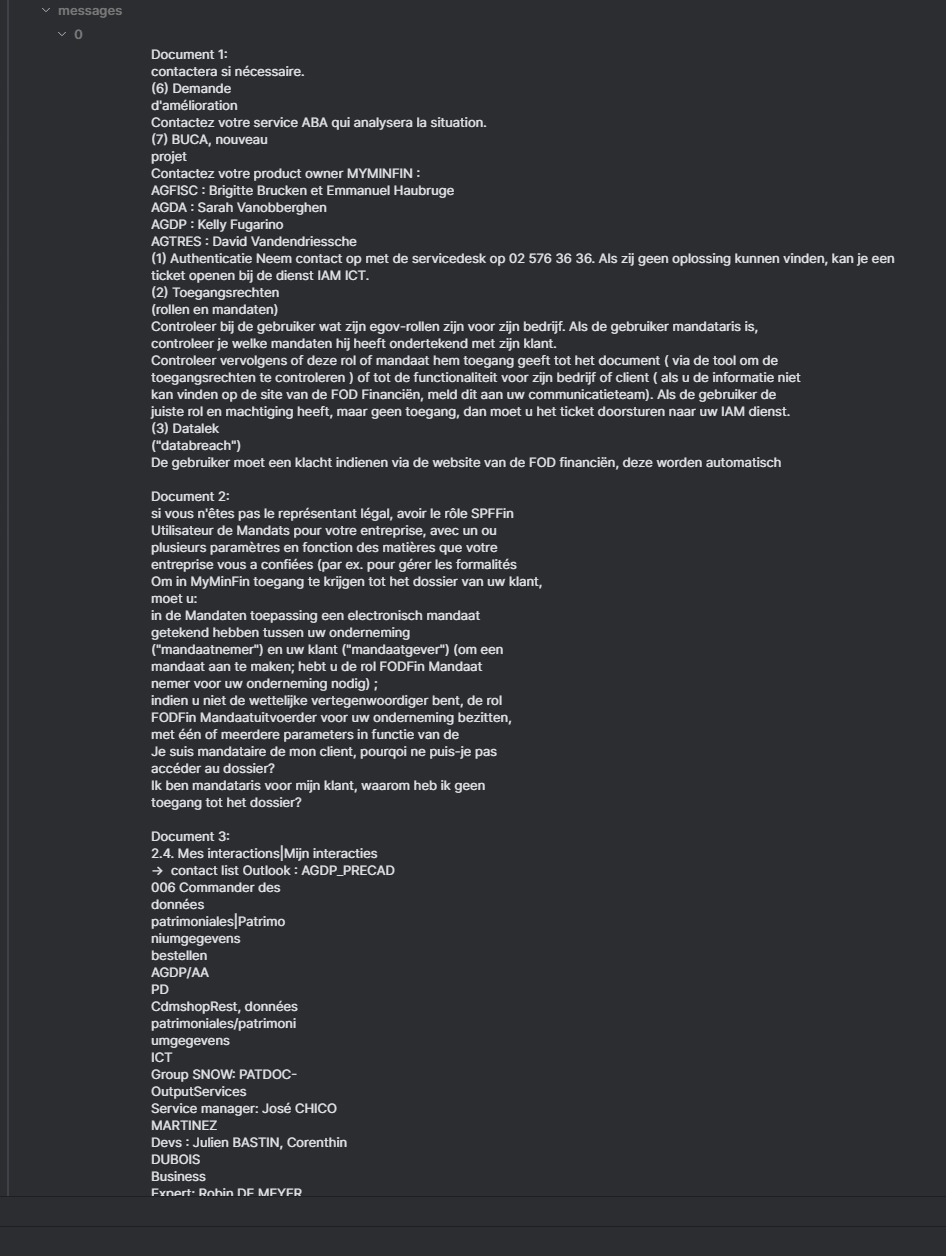
\includegraphics[width=\linewidth]{chunks_pdf.png}
        \caption{Chunks in PDF}
        \label{fig:chunks_pdf}
    \end{subfigure}
    \hfill
    \begin{subfigure}{0.3\textwidth}
        \centering
        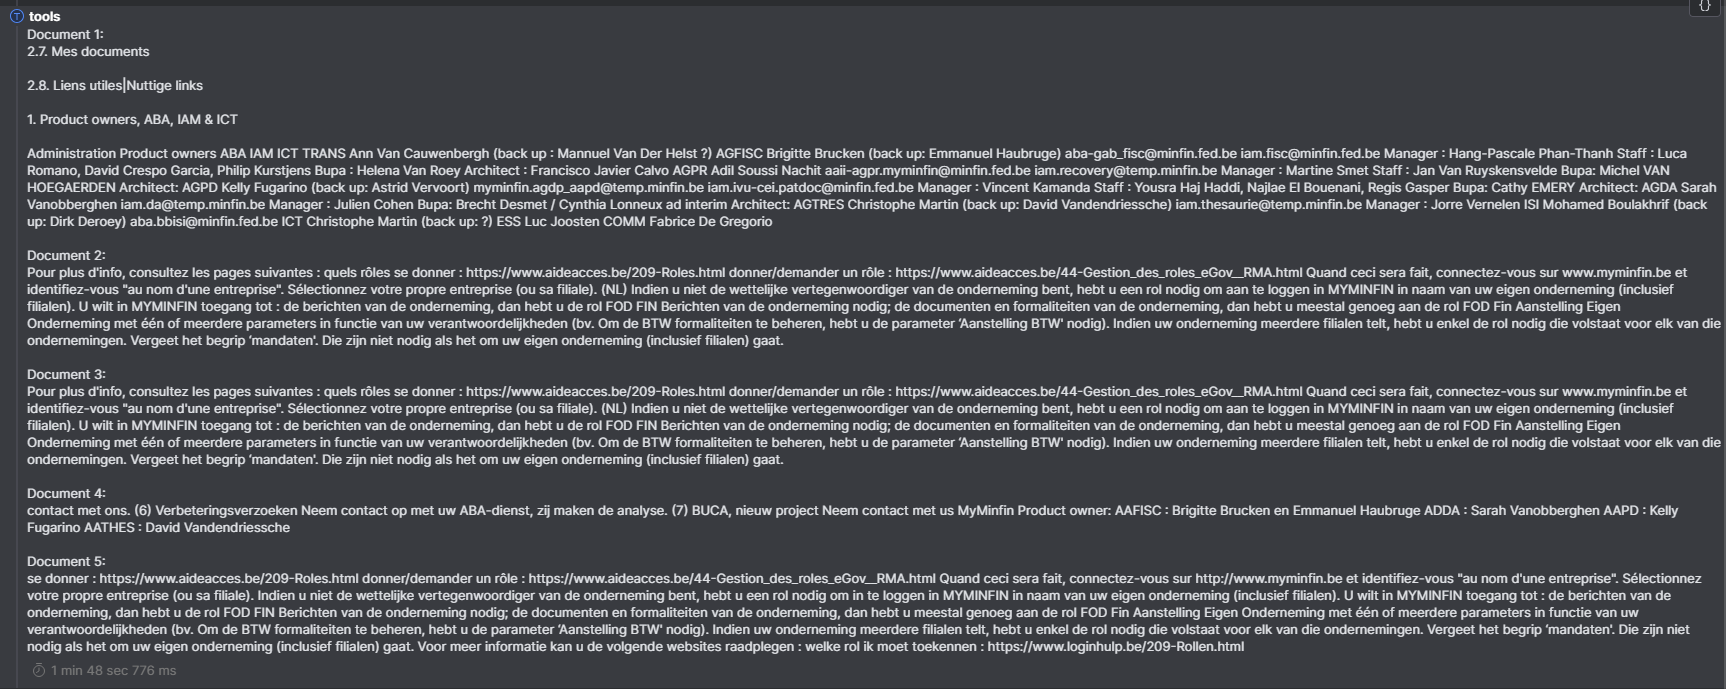
\includegraphics[width=\linewidth]{chunks_docx.png}
        \caption{Chunks in DOCX}
        \label{fig:chunks_doc}
    \end{subfigure}
     \hfill
    \begin{subfigure}{0.3\textwidth}
        \centering
        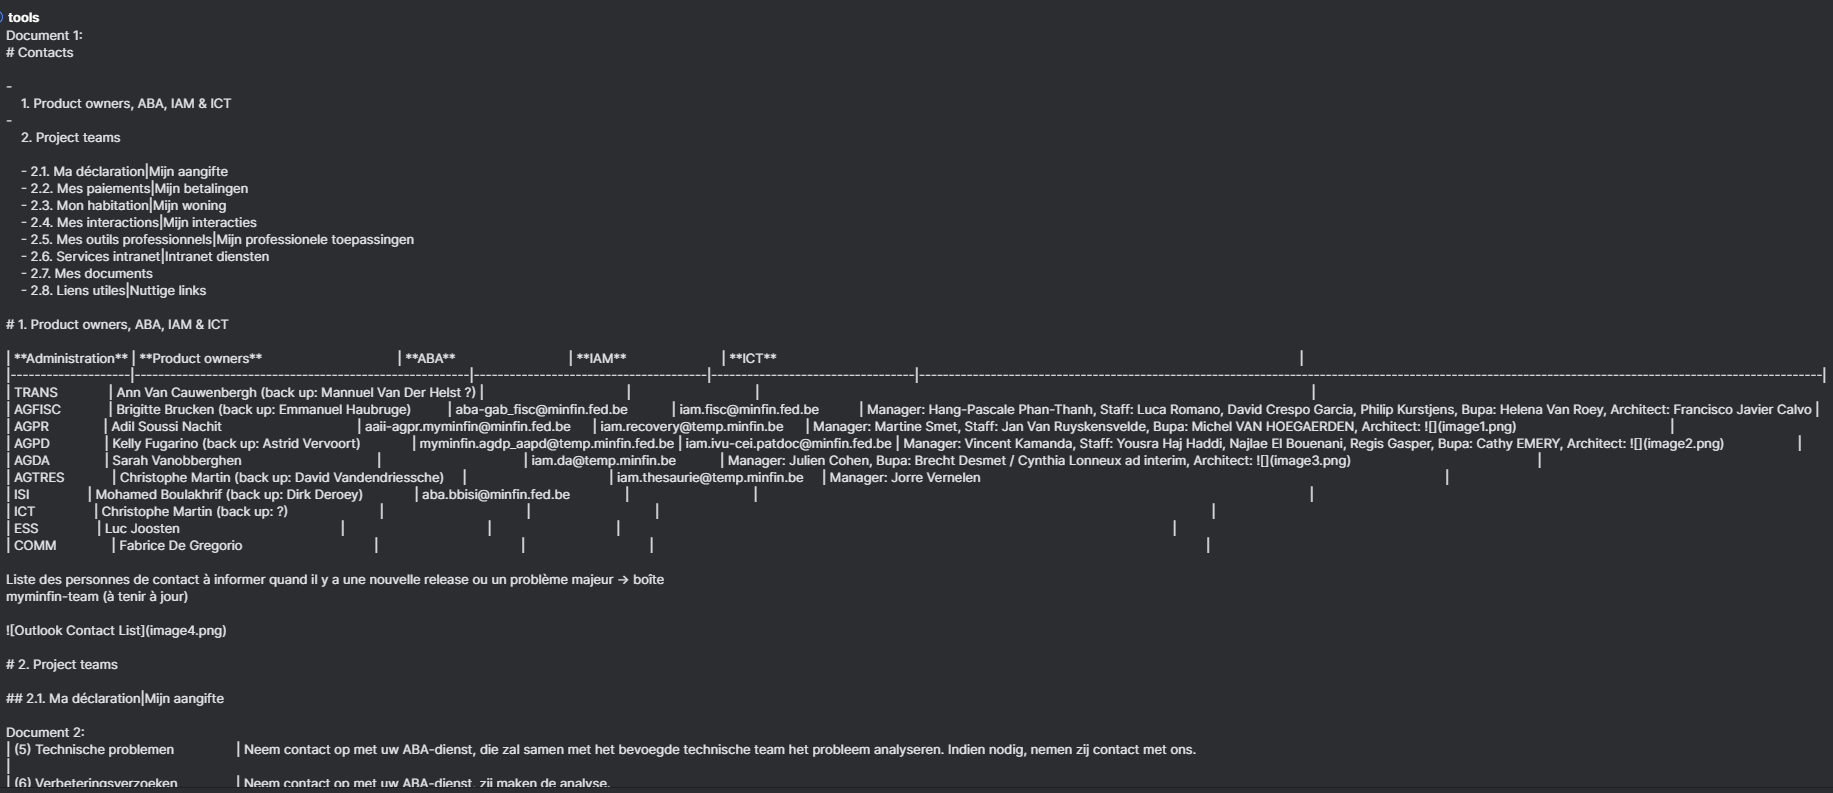
\includegraphics[width=\linewidth]{chunks_md.png}
        \caption{Chunks in Markdown}
        \label{fig:chunks_md}
    \end{subfigure}
    \caption{Chunks per document type}
    \label{fig:driefiguren}
\end{figure}

\subsection{Tool calls}

Omdat er in de graaf gebruik wordt gemaakt van een tool, is het noodzakelijk om modellen te gebruiken die in staat zijn om tool-calls uit te voeren. Hierdoor is het in deze PoC bijvoorbeeld niet mogelijk om met Google's Gemma modellen te werken, aangezien deze LLM-modellen geen ondersteuning bieden voor tool-calls.
\\[1em]
Hoewel sommige Ollama modellen wel tool-calls ondersteunen, blijkt uit de praktijk dat deze functionaliteit niet altijd betrouwbaar is. Ondanks dat de modellen technisch gezien tool-calls kunnen uitvoeren, levert dit niet altijd het gewenste resultaat op.
\\[1em]
Bij het bepalen van de modellen voor de vergelijkende studie werd dan ook vastgesteld dat testen met een aantal modellen onmogelijk was, omdat de vereiste tool-call naar de retriever simpelweg niet werd gegenereerd. 

\begin{figure}[H]
    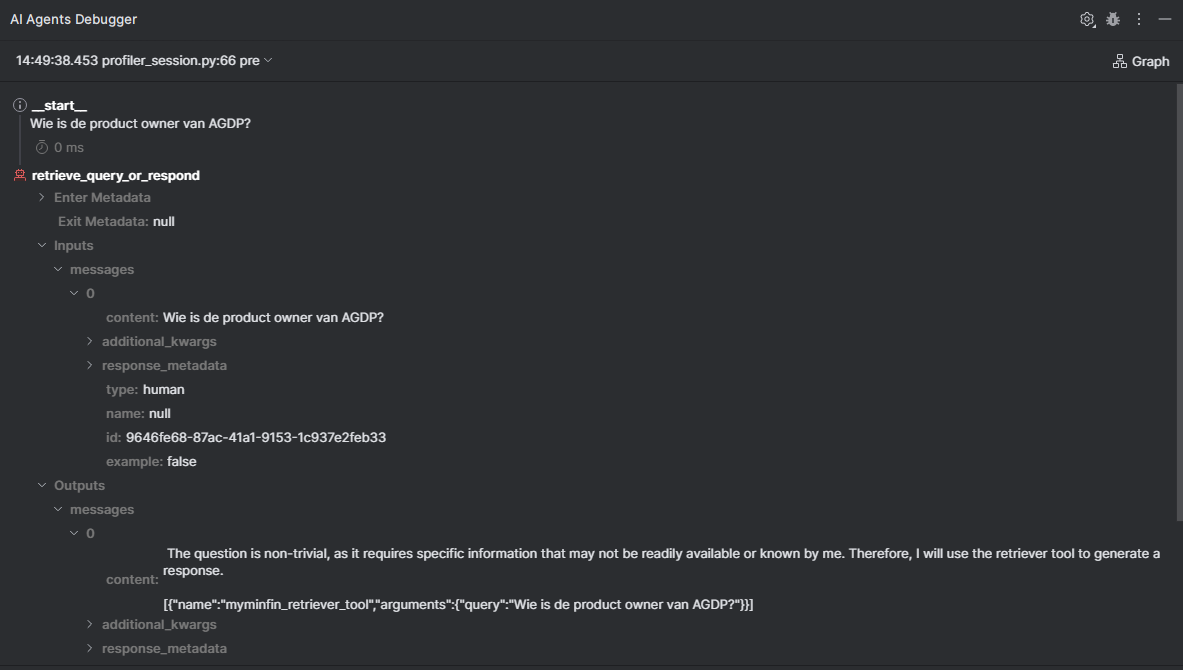
\includegraphics[width=0.8\textwidth]{mistral.png}
    \caption{Tool call bij het Mistral:7b model}
    \label{fig:Mistral}
\end{figure}

De figuur~\ref{fig:Mistral} illustreert waar het fout loopt bij dit model. Ondanks dat het model zich bewust is van de aanwezigheid van de tool en correct inschat dat de gestelde vraag niet triviaal is, wordt de tool-call toch niet effectief uitgevoerd.
\\[1em]
Opmerkelijk is dat de tool-call met de juiste parameters wel aanwezig is in de content van het antwoord, maar deze wordt niet als daadwerkelijke tool-call geïnterpreteerd of geactiveerd door het model.
\\[1em]
Dit probleem deed zich voor bij meerdere modellen. Daardoor kunnen deze modellen niet worden gebruikt binnen deze PoC en de bijhorende vergelijkende studie, aangezien ze de vectordatabase nooit aanspreken en dus geen relevante antwoorden aan de gebruiker kunnen bieden.

\subsection{Fout door oneindige herformuleringslus}

Hoewel de LLM in staat is om zelf te bepalen wat een non triviale vraag is, betekent dit niet noodzakelijk dat het antwoord daarop terug te vinden is in de beschikbare documentatie. Zelfs wanneer de informatie wel aanwezig is, kan het alsnog voorkomen dat de LLM, zelfs na herformulering van de vraag, geen passend antwoord weet te genereren. Dit leidde aanvankelijk tot een oneindige lus waarbij uiteindelijk een foutmelding werd gegenereerd zodra de array messages in de MessageState een lengte van 25 bereikte. In dat geval werd er geen antwoord aangemaakt, maar kreeg de gebruiker enkel een foutmelding te zien met stacktrace.
\\[1em]
Om te voorkomen dat het programma in een dergelijke oneindige lus terechtkomt, werd er een extra controle ingebouwd op het moment dat de LLM moet kiezen tussen het herformuleren van de vraag of het genereren van een antwoord. In de praktijk betekent deze controle dat de LLM de vraag maximaal twee keer mag herformuleren. Hierdoor wordt de vectordatabase in totaal maximaal drie keer bevraagd. Indien er na deze pogingen nog steeds geen relevante documenten worden teruggevonden, is het de bedoeling dat de LLM dit expliciet communiceert aan de gebruiker, zonder dat er sprake is van hallucinaties. 

\subsection{Meertaligheid documentatie}
%het gaat hier over het feit dat hij steeds de eerste vraag vertaalde naar het engels.
%Hoe heb je dat opgelost? Eventueel kort uitleggen als dat relevant is.
Bij het testen van de lus ontstond het probleem dat telkens enkel de originele vraag werd herschreven. Hierdoor werd bijvoorbeeld de oorspronkelijke vraag wel correct naar het Engels herschreven, maar bij iedere volgende iteratie werd opnieuw exact dezelfde vertaling gegenereerd. Er werd met vorige pogingen geen rekening gehouden.
\\[1em]
Om dit probleem op te lossen, werd de prompt in de \verb|rewrite_question| node aangepast zodat de LLM ook rekening kan houden met de eerder gestelde en herschreven vragen. Dit voorkomt herhaling en zorgt voor meer variatie in de gegenereerde vragen.
\\[1em]
Aangezien het grootste deel van de beschikbare documentatie in het Frans of Engels is geschreven, wordt de LLM eveneens aangemoedigd om de vraag eerst naar het Frans te herschrijven en vervolgens, indien nodig, naar het Engels.

\begin{lstlisting}[basicstyle=\small, frame=single, breaklines=true, postbreak=\mbox{\textcolor{red}{$\hookrightarrow$}\space}, escapeinside ={\%,}, escapechar={!}, numbers=left, language=Python, caption=Beoordeling documenten prompt]
REWRITE_QUESTION_PROMPT = (
    "You are assisting with improving a user's question related to Myminfin IT support.\n"
    "Conversation history so far (most recent last):"
    "\n ------- \n"
    "{questions}"
    "\n ------- \n"
    "Original question:"
    "\n ------- \n"
    "{original_question}"
    "\n ------- \n"
    "Rewrite the last question to make it short, clear, and easy to match with relevant documents in a vector database.\n"
    "- Keep the meaning and intent exactly the same.\n"
    "- Use simple, direct wording without adding unnecessary details.\n"
    "- If the question is in Dutch, rewrite and translate it to French.\n"
    "- If the question is in French, rewrite and translate it to English.\n"
    "- Avoid repeating previous questions word-for-word.\n"
    "- If it’s similar to a previous question, add only minimal context needed for distinction.\n"
    "- Return only the rewritten question."
)
\end{lstlisting}
\section{Samenvatting}

%Korte recap: wat is gebouwd en werkt zoals verwacht?
%Eventueel: wat is nog niet geïmplementeerd en waarom niet (scope, tijdsbeperkingen)?

Het eindresultaat van deze PoC is een chatinterface die kan worden gebruikt om gerichte vragen te stellen aan de IT-support voor MyMinfin. De toepassing werkt zoals verwacht: afhankelijk van de vraag worden relevante documenten opgehaald en wordt de nodige informatie aan de eindgebruiker verstrekt. Hoewel de hoeveelheid documentatie nog verder opgeschaald kan worden, vormt dit een sterke eerste stap in het opzetten van een ondersteunende tool voor de dagelijkse supportwerking.
\\[1em]
Toch zijn er ook enkele zaken die momenteel nog ontbreken. Zo zou het nuttig zijn indien de agent zelfstandig documentatie kan aanpassen of aanvullen. Dit zou ervoor zorgen dat de beschikbare informatie steeds up-to-date blijft, zonder dat hiervoor handmatige tussenkomst van gebruikers nodig is. Deze functionaliteit viel echter buiten de scope van deze PoC en kon, omwille van tijdsbeperkingen, niet worden gerealiseerd.
\\[1em]
Daarnaast beschikt de huidige LLM-toepassing niet over enige vorm van geheugen. Bij elke nieuwe vraag begint de LLM volledig van nul, zonder kennis van eerdere interacties binnen dezelfde sessie. Er is dus geen sprake van contextopbouw of het onthouden van vorige vragen en antwoorden, wat de gebruikservaring momenteel beperkt tot losstaande interacties.